\documentclass[12pt]{article}

%Packages:
\usepackage[utf8]{inputenc}    
\usepackage[vietnamese]{babel} 
\usepackage{graphicx}          
\usepackage{amsmath , amsfonts , amssymb , amsthm} 
\usepackage{hyperref}          
\usepackage{geometry}    
\usepackage{framed}
\usepackage{float}
\usepackage{array}
\usepackage{multirow}
\usepackage{pgfplots}
\usepackage[version=4]{mhchem}
\usepackage{fancyhdr}
\usepackage{lastpage} % để lấy tổng số trang
\pagestyle{fancy}
\fancyhf{}
\renewcommand{\footrulewidth}{0.4pt}

\fancyfoot[L]{Báo cáo thí nghiệm Hoá đại cương nhóm 6 - HK242.}

% Chân trang bên phải
\fancyfoot[R]{Trang \thepage/\pageref{LastPage}}

\begin{document}
%Trang bìa
\begin{titlepage}
    \centering
    {\textbf{ĐẠI HỌC QUỐC GIA THÀNH PHỐ HỒ CHÍ MINH}} \\   
    {\textbf{TRƯỜNG ĐẠI HỌC BÁCH KHOA}} \\   
%Chèn logo BK    
\begin{figure}[h]
    \centering
    
\includegraphics[width=0.4\textwidth]{img/Bach khoa.png}
\end{figure}
%Title
    {\huge \textbf{BÁO CÁO THÍ NGHIỆM  }} \\
    {\huge \textbf{HOÁ ĐẠI CƯƠNG}} \\
    \hrulefill \\
    \vspace{0.5cm}
    
    { \textbf{GVHD: Trần Thị Thanh Thuý}} \\
    { \textbf{Nhóm: 6}} \\
    \vspace{0.5cm}

\begin{tabular}{|m{1cm}|m{3cm}|m{3cm}|m{2cm}|}
\hline
STT & Họ và đệm  & Tên &  MSSV \\ \hline
1 & Nguyễn Thái & Hưng & 0000000 \\ \hline
\end{tabular}
\vspace{6cm} \\
\textbf{Thành phố Hồ Chí Minh, tháng 6 năm 2025}
\end{titlepage}

%Muc luc
\tableofcontents
\newpage
\section{Lời nói đầu}
{\Large Lời đầu tiên, nhóm em xin gửi lời cảm ơn chân thành nhất đến giảng viên bộ môn thí nghiệm Hoá đại cương là cô Trần Thị Thanh Thuý đã hướng dẫn và hỗ trợ trong quá trình thực hiện các bài thí nghiệm và bài báo cáo lần này. Thông qua quá trình thực hiện thí nghiệm, chúng em đã được bổ sung thêm nhiều kiến thức và có cơ hội được thí nghiệm thực tế. Đó là những tri thức quý báu.\\
Được sự phân công của cô, nhóm em xin trình bày bài báo cáo của các bài thí nghiệm 2,4 và 8 theo chương trình giảng dạy. Trong bài báo cáo này, nhóm em sẽ trình bày cách thức thực hiện các bài thí nghiệm, cũng như xử lý các số liệu thu được trong quá trình thí nghiệm và trả lời các câu hỏi được đặt ra theo mẫu báo cáo.\\
Nhờ việc thực hiện bài báo cáo này, em được củng cố lại kiến thức. Nhưng kiến thức về môn Hoá đại cương vẫn còn nhiều hạn chế nên chắc chắn bài báo cáo vẫn còn thiếu sót khó tránh. Vì thế chúng em sẵn sàng nhận được sự góp ý và lắng nghe phản hồi của cô để giúp chúng em hoàn thiện hơn.\\
\begin{center}
    Chúng em xin chân thành cảm ơn!
\end{center}
}
\newpage
\section{Bảng số liệu thực tế}
\begin{figure}[H]
    \centering
    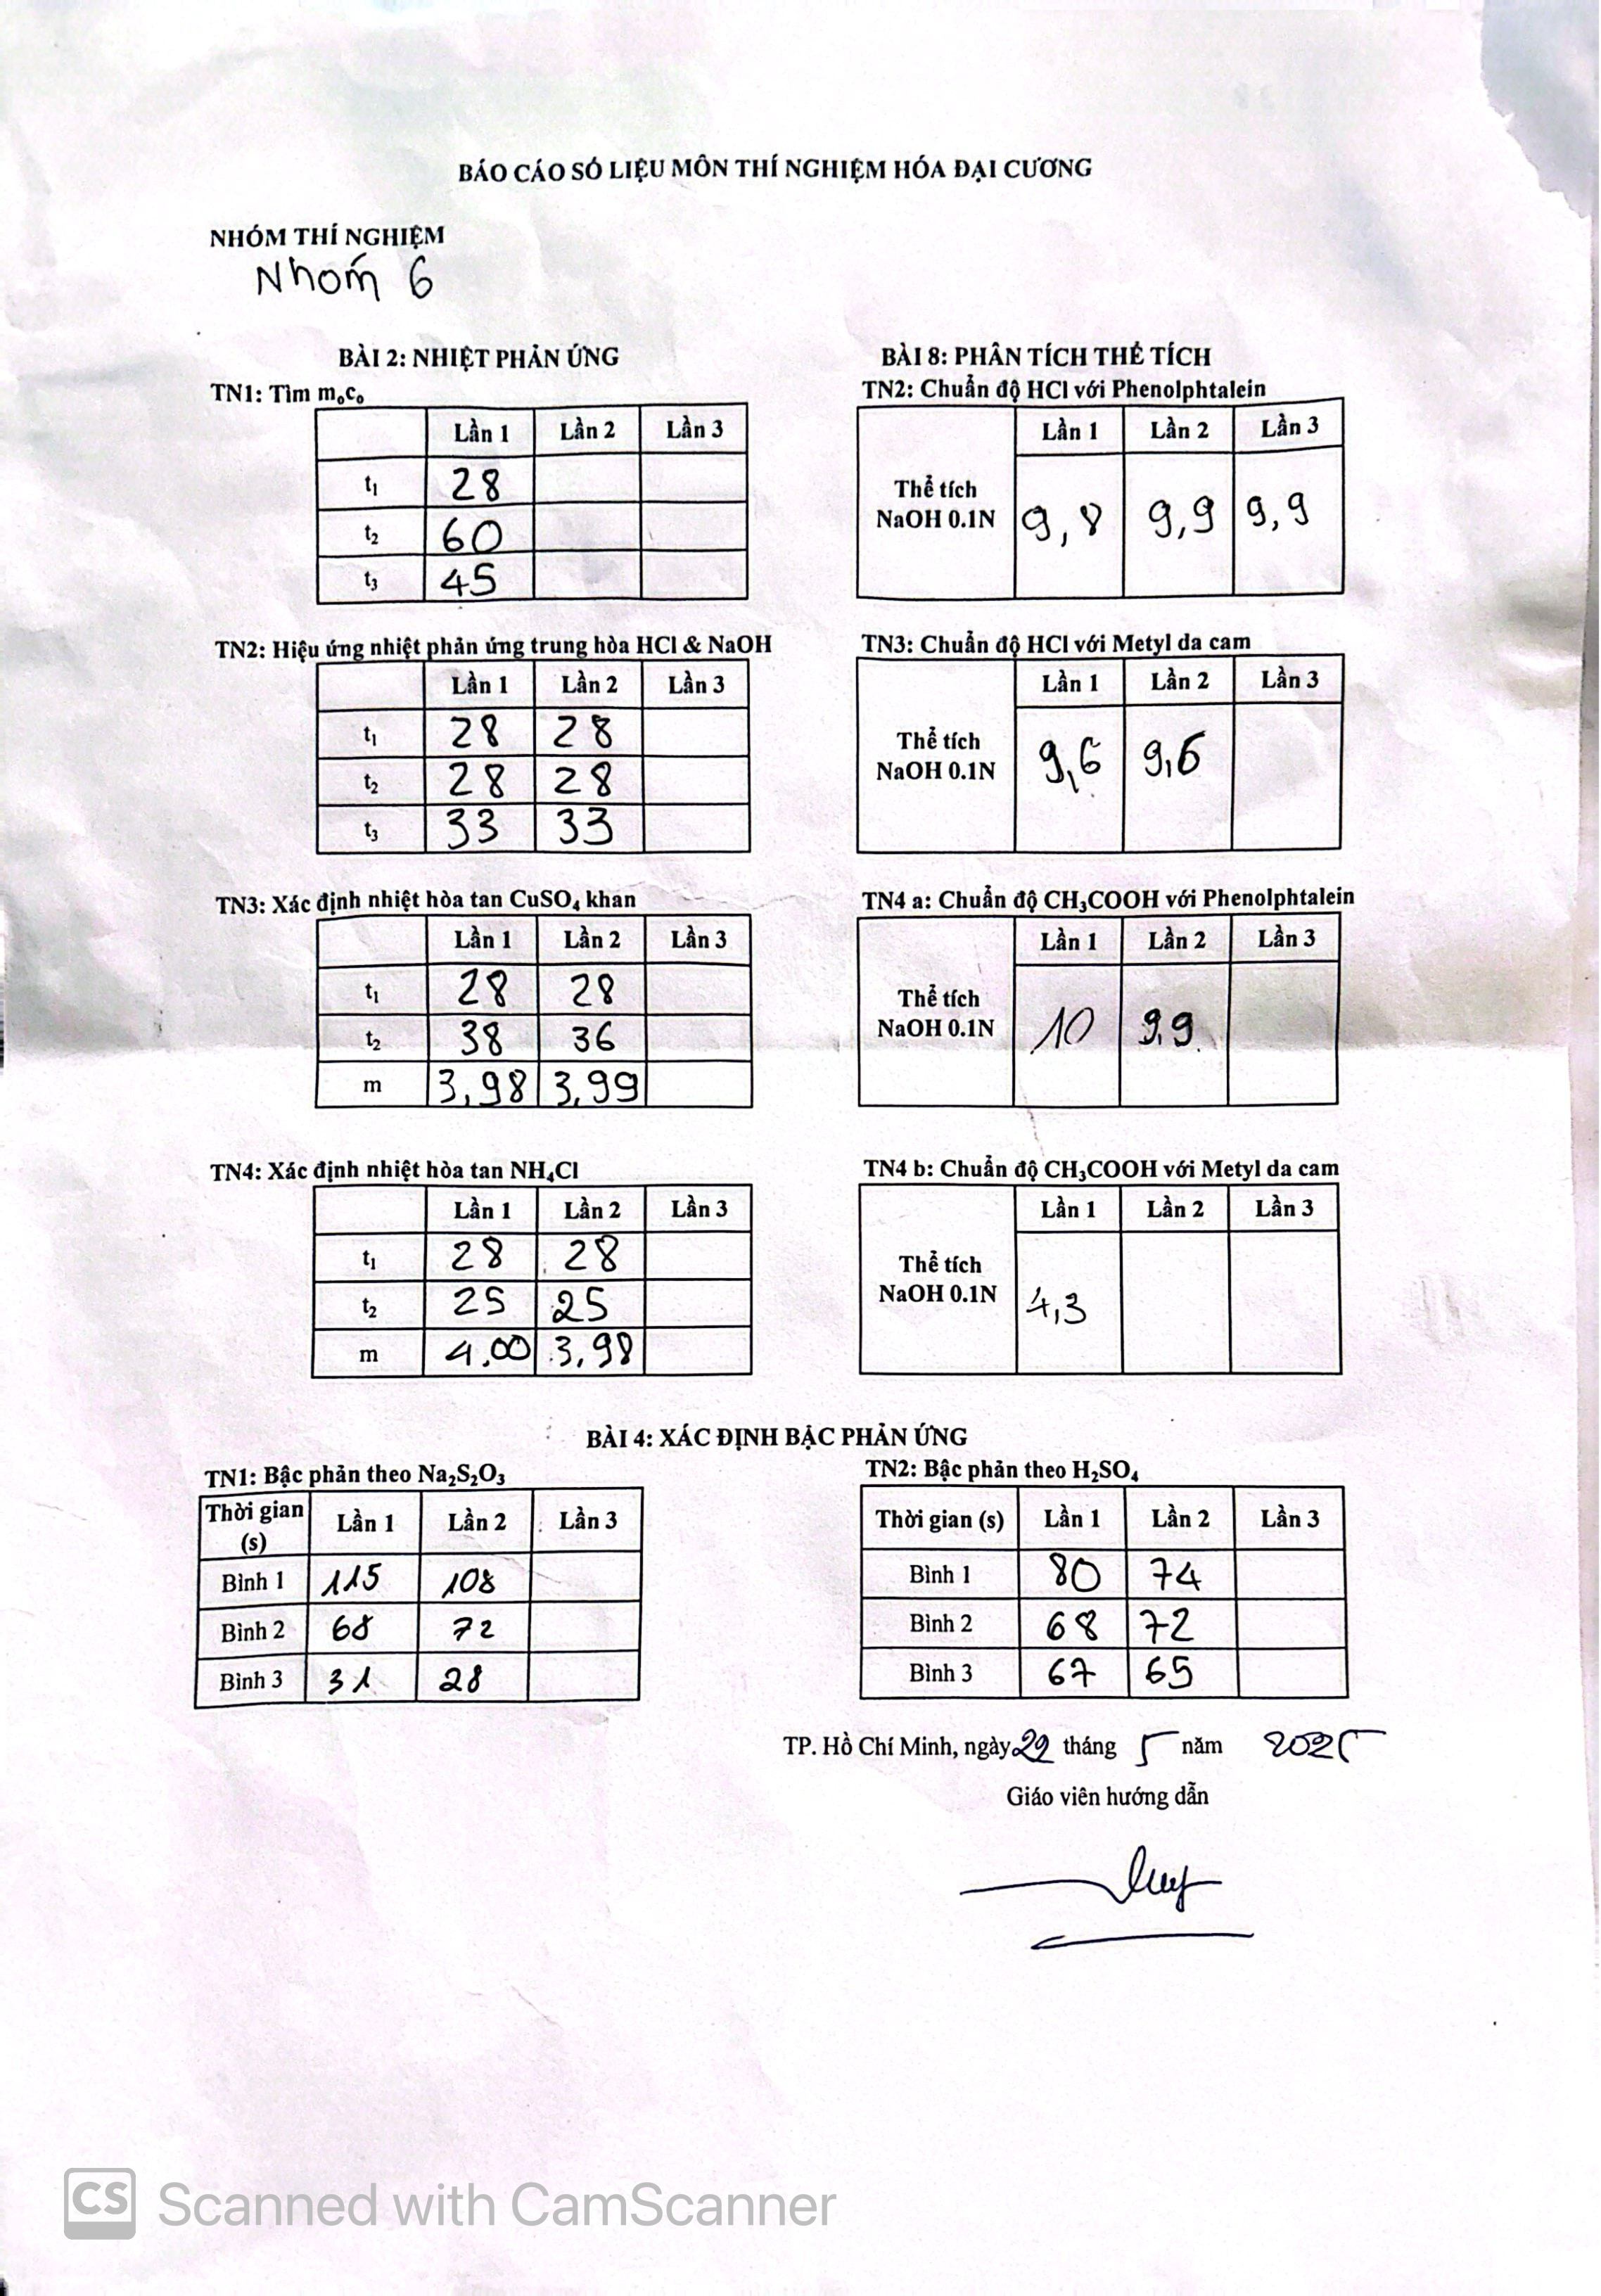
\includegraphics[scale=0.15]{img/Baocaosolieu.jpeg}
    \caption{Bảng số liệu thu được từ thí nghiệm}
    \label{fig:enter-label}
\end{figure}
\newpage
%BAI 2: NHIET PHAN UNG
\section{Bài 2: Nhiệt phản ứng}
\subsection{Tiến hành thí nghiệm}
\subsubsection{Thí nghiệm 1: Xác định nhiệt dung bằng nhiệt lượng kế}
Thí nghiệm này chỉ làm 1 lần.
Đặt ống đong trên mặt phẳng cố định rồi cho nước cất vào (đặt mắt phải ngang
với vạch 50ml và mặt cong nhất phải chạm vạch 50) $\rightarrow$ cho vào cốc cắm nhiệt
kế và đo nhiệt độ $t_1 \rightarrow$ lấy ống đong xong lấy tiếp 50ml nước nóng và cho vào bình nhiệt lượng kế cắm nhiệt kế và đo nhiệt độ $t_2 \rightarrow$ rửa và lau khô nhiệt kế để trả về nhiệt độ phòng (bắt buộc) $\rightarrow$ mở nút ra lắp phễu rót phần nước nguội trong cốc vào trong bình nhiệt lượng kế rồi lấy phễu ra lắp nhiệt lượng kế rồi lấy phễu ra lắp nhiệt kế lên $\rightarrow$ lắc đều cho nước nóng và nước thường trao đổi nhiệt và xác định nhiệt độ $t_3$.
\subsubsection{Thí nghiệm 2: Xác định hiệu ứng nhiệt của phản ứng trung hoà HCl và NaOH}
Đầu tiên rửa cây buret, cây buret nào chứa hóa chất nào thì tráng bằng hóa chất
đó $\rightarrow$ đóng khóa buret bằng tay trái đổ hóa chất lên đầy cây buret và chỉnh cây buret ( phải làm hết bọt khí và chỉnh buret về 0) $\rightarrow$ →mở khóa buret chứa dung dịch NaOH (lấy 25ml, chú ý không xả hết cây buret) lên đầy cây buret và chỉnh (phải làm hết bọt khí và chỉnh buret về 0) $\rightarrow$ mở khóa buret chứa dung dịch NaOH (lấy 25ml, chú ý không xả hết cây buret) $\rightarrow$ cắm nhiệt kế vào cốc chứa NaOH xác định nhiệt độ $t_1 \rightarrow$ lấy bình nhiệt lượng kế ra cho dưới cây HCl, lấy 25ml dung dịch HCl cho vào bình nhiệt lượng kế $\rightarrow$ rửa và lau khô, trả nhiệt kế về nhiệt độ phòng rồi mới cắm vào bình nhiệt lượng kế đo nhiệt độ $t_2 \rightarrow$ lắp phễu lên rót phần NaOH từ trong cốc vào trong bình nhiệt lượng kế, lấy phễu ra và đóng nút lại, lắc đều lên đo nhiệt độ $t_3$.
\subsubsection{Thí nghiệm 3: Xác định nhiệt hoà tan \ce{CuSO4} khan}
Dùng ống đong lấy 50ml nước cất cho vào bình nhiệt lượng kế, cắm nhiệt kế
vào đo nhiệt độ $t_1$ → cân nhanh gần bằng 4g \ce{CuSO_4} khan, ghi lại khối lượng
đó → mở hẳn nắp bình nhiệt lượng kế, trút phần chất rắn vào → đậy nắp lại, lắp nhiệt kế và lắc đều (nhiệt tỏa ra là nhiệt hòa tan của \ce{CuSO_4} vào nước), xem
nhiệt độ lên cao nhất (cực đại) rồi sau đó giảm lấy nhiệt độ cao nhất (cực đại) là
$t_2$.
\subsubsection{Thí nghiệm 4: Xác định nhiệt hoà tan \ce{NH_4Cl}}
Dùng ống đong lấy 50ml nước cất cho vào bình nhiệt lượng kế cắm nhiệt kế
vào và đo nhiệt độ $t_1$→ cân nhanh gần bằng 4g \ce{NH_4Cl} và ghi lại khối lượng đó
→ mở hẳn nắp bình nhiệt lượng kế ra và trút phần chất rắn vào → đậy nắp lại, lắp nhiệt kế lên và lắc đều (nhiệt tỏa ra là nhiệt hòa tan của \ce{NH_4Cl} vào nước), xem nhiệt độ lên cao nhất (cực đại) rồi sau đó giảm lấy nhiệt là $t_2$.
\newpage
\subsection{Kết quả thí nghiệm}
\subsubsection{Thí nghiệm 1: Xác định nhiệt dung bằng nhiệt lượng kế}
{\centering \begin{tabular}{|m{3cm}|m{3cm}|}
\hline
Nhiệt độ  & Lần 1  \\ \hline
$t_1$ & 28   \\ \hline
$t_2$& 60   \\ \hline
$t_3$ & 45  \\ \hline
$m_0c_0 (cal/^\circ\mathrm{C}) $ & 6.6667 \\ \hline
\end{tabular} \\} \\
Ta có:
\[
\begin{cases}
m  = 50(g)\\
c =  1 (cal/g^\circ\mathrm{C})
\end{cases} 
\rightarrow mc = 50 \cdot 1  = 50 (cal/^\circ\mathrm{C})
\]
Từ đó, ta thu được:
\[
m_0c_0 = mc \cdot \frac{(t_3 -t_1) - (t_2 - t_3)}{t_2 - t_3} =  50 \cdot \frac{(45-28) - (60 -45)}{60 -45} = \frac{20}{3}= 6.6667 (cal/^\circ\mathrm{C})
\] 


\subsubsection{Thí nghiệm 2: Xác định hiệu ứng nhiệt của phản ứng trung hoà HCl và NaOH}
{\centering \begin{tabular}{|m{3cm}|m{3cm}|m{3cm}|}
\hline
  & Lần 1 & Lần 2 \\ \hline
$t_1$ & 28 & 28 \\ \hline
$t_2$& 28 & 28 \\ \hline
$t_3$ & 33 & 33\\ \hline
Q(cal) &288.3333 & 288.3333\\ \hline
\(Q_{\text{tb}}\) (cal) & \multicolumn{2}{c|}{288.3333} \\ \hline
$\Delta H$ (cal/mol) & \multicolumn{2}{c|}{-11533.332} \\ \hline
\end{tabular}\\  } 
Ta có:\\
\[
m_{NaCl}c_{NaCl} = (V_{NaOH} + V_{HCl})\cdot1.02 = (25 + 25) \cdot 1.02 = 51 (cal/^\circ\mathrm{C})
\]
\[
Q_1 = (m_0c_0 + m_{NaCl}c_{NaCl})\cdot(t_3 - \frac{t_1 +t_2}{2})
\]
\[
Q_1 = Q_2 = (6.6667+ 51) \cdot (33 - \frac{28 + 28}{2}) = 288.3333 (cal)
\]
\[
Q_{tb} = \frac{Q_1 + Q_2}{2} = \frac{288.3333 + 288.3333}{2} = 288.3333 (cal)
\]
\[
\Delta H = - \frac{Q_{tb}}{n} = - \frac{288.3333}{0.025} = -11533.332 (cal/mol)
\] 
Do $\Delta H < 0$ nên phản ứng toả nhiệt.
\newpage
\subsubsection{Thí nghiệm 3: Xác định nhiệt hoà tan CuSO$_4$ khan}
{\centering \begin{tabular}{|m{3cm}|m{3cm}|m{3cm}|}
\hline
  & Lần 1 & Lần 2 \\ \hline
$t_1$ & 28 & 28 \\ \hline
$t_2$& 38 & 36 \\ \hline
$m$ & 3.98 & 3.99\\ \hline
Q(cal) & 606.4667 & 485.2536\\ \hline
$\Delta H$ (cal/mol) & -24380.5709 & -19507.6824 \\ \hline
$\Delta H_{tb}$ (cal/mol) & \multicolumn{2}{c|}{-21944.1267} \\ \hline
\end{tabular}\\  } 
Ta có: \\
$c_{CuSO_4} = 1 (cal/g^\circ\mathrm{C})$ ;
$M_{CuSO_4} = 160(g/mol)$ ;\\
$m_{nước} = 50g$ ;
$c_{nước} = 1 (cal/g^\circ\mathrm{C}) $ (Trong đó: nc viết tắt cho nước cất)
\[
n_{CuSO_4} = \frac{m_{CuSO_4}}{M_{CuSO_4}} = \frac{3.98}{160}= 0.024875 (mol)
\]
\[
Q_1 = mc \Delta t = ( m_0c_0 + m_{nước}c_{nước} + m_{CuSO_4}c_{CuSO_4}) \cdot (t_2 - t_1)
\]
\[
Q_1 = (6.6667 + 50 + 3.98) \cdot (38-28) = 606.4667 (cal)
\]
\[
\Delta H_1 = - \frac{Q_1}{n} = - \frac{606.4667}{0.024875} = -24380.5709 (cal/mol)
\]
Tính tương tự cho lần 2, ta có:
\[
Q_2 = (6.6667 + 50 +3.99) \cdot (36-28) = 485.2536 (cal)
\]
\[
\Delta H_2 = -\frac{Q_2}{n} = -\frac{485.2536}{0.024875} = - 19507.6824 (cal/mol)
\]
Từ đó ta có:
\[
\Delta H_{tb} = \frac{\Delta H_1 + \Delta H_2}{2} = \frac{-24380.5709-19507.6824}{2}= -21944.1267 (cal/mol)
\]
Do $\Delta H_{tb} < 0 $ nên phản ứng toả nhiệt. 
\subsubsection{Thí nghiệm 4: Xác định nhiệt hoà tan của NH$_4$Cl}
{\centering \begin{tabular}{|m{3cm}|m{3cm}|m{3cm}|}
\hline
  & Lần 1 & Lần 2 \\ \hline
$t_1$ & 28 & 28 \\ \hline
$t_2$& 25 & 25 \\ \hline
$m$ & 4.00 & 3.98 \\ \hline
Q(cal) &-182.0001  & -181.9401\\ \hline
$\Delta H$ (cal/mol) & 2433.1564 &  2432.3542 \\ \hline
$\Delta H_{tb}$ (cal/mol) & \multicolumn{2}{c|}{2432.7553} \\ \hline
\end{tabular}\\  } 
\newpage
\[
n_{NH_4Cl} = \frac{m_{NH_4Cl}}{M_{NH_4Cl}} = \frac{4}{53.5} = 0.0748 (mol)
\]
\[
Q_1 = mc \Delta t = ( m_0c_0 + m_{nước}c_{nước} + m_{NH_4Cl}c_{NH_4Cl}) \cdot (t_2 - t_1)
\]
\[
Q_1 = (6.6667 +50+4) \cdot (25 -28)= -182.0001 (cal)
\]
\[
\Delta H_1 = - \frac{Q_1}{n} = - \frac{-182.0001}{0.0748} = 2433.1564 (cal/mol)
\]
Tính tương tự cho lần 2, ta có:
\[
Q_2 = (6.6667 + 50 + 3.98)\cdot (25-28) = -181.9401 (cal)
\]
\[
\Delta H_2 = -\frac{Q_2}{n} = - \frac{-181.9401}{0.0748} = 2432.3542 (cal/mol)
\]
Từ đó ta thu được:
\[
\Delta H_{tb} = \frac{\Delta H_1 + \Delta H_2}{2} = \frac{2433.1564 +2432.3542 }{2 } = 2432.7553 (cal/mol)
\]
Do $\Delta H_{tb} > 0 $ nên phản ứng thu nhiệt.
\subsection{Trả lời câu hỏi}
\textbf{Câu 1: }$\Delta H_{th}$ của phản ứng \ce{HCl + NaOH \rightarrow NaCl + H_2O} sẽ được tính theo số mol HCl hay NaOH khi cho 25ml dung dịch HCl 2M tác dụng với 25 ml dung dịch NaOH 1M? Tại sao?


    \textbf{Trả lời:} \\
$n_{NaOH} = 1 \cdot 0.025 = 0.025 (mol)$ \\
$n_{HCl} = 2  \cdot 0.025 = 0.05 (mol)$

Ta có phản ứng:
\[
\begin{array}{lcccccc}
& \ce{HCl & + & NaOH & \rightarrow & NaCl & + H_2O} \\
\text{Ban đầu (mol)} & 0.05 & & 0.025 & & 0.025 & 0.025 \\
\text{Phản ứng (mol)} & 0.025 & & 0.025 & & 0.025 & 0.025 \\
\text{Còn lại (mol)} & 0.025 & & 0 & & 0.025 & 0.025 \\
\end{array}
\]
\begin{itemize}
    \item Vì NaOH hết và HCl dư nên $\Delta H_{\text{th}}$ của phản ứng tính theo NaOH.
    \item Lượng HCl dư chỉ làm môi trường, không tham gia phản ứng do đó không sinh nhiệt.
\end{itemize}
\textbf{Câu 2:} Nếu thay HCl 1M bằng HNO$_3$ 1M thì kết quả thí nghiệm 2 có thay đổi hay không?


\textbf{Trả lời:} \\
Phương trình 1:

\[
\ce{HCl + NaOH -> NaCl + H2O}
\]
\[
\ce{H+  + OH^- -> H2O}
\]
Phương trình 2:
\[
\ce{HNO3 + NaOH -> NaNO3 + H2O}
\]
\[
\ce{H+ + OH^-  -> H2O}
\]
\begin{itemize}
    \item Kết quả thí nghiệm 2 không thay đổi do HCl và HNO$_3$ là hai axit mạnh phân ly hoàn toàn. Đồng thời, phản ứng ở thí nghiệm 2 là phản ứng trung hoà.
    \item Khi thay vào công thức $Q = mc\Delta t$, mặc dù $m$ và $c$ thay đổi nhưng biến đổi đều, nên $Q$ và $\Delta H$ không đổi.
\end{itemize}
\textbf{Câu 3:} Tính $\Delta H_3$ bằng lý thuyết theo định luật Hess. So sánh với kết quả thí nghiệm. Hãy xem 6 nguyên nhân có thể gây ra sai số trong thí nghiệm này:
\begin{enumerate}
    \item Mất nhiệt do nhiệt lượng kế.
    \item Do nhiệt kế.
    \item Do dụng cụ đong thể tích hóa chất.
    \item Do cân.
    \item Do sunfat đồng bị hút ẩm.
    \item Do lấy nhiệt dung riêng dung dịch sunfat đồng bằng 1 cal/mol.độ.
\end{enumerate}
Theo em, sai số nào là quan trọng nhất? Còn nguyên nhân nào khác không?


\textbf{Trả lời:} \\
Theo định luật Hess:
\[
\Delta H_3(\text{lt}) = \Delta H_1 + \Delta H_2 = -18{,}7 + 2{,}8 = -15{,}9 \ (\text{kcal/mol}) = -15900 \ (\text{cal/mol})
\]
Theo thực nghiệm:
\[
\Delta H_3(\text{tn}) = -21944.1267\ (\text{cal/mol})
\]

$\Rightarrow$ Chênh lệch tương đối. \\
Nhận xét về sai số:
\begin{itemize}
    \item Theo em, trong 6 nguyên nhân trên, nguyên nhân quan trọng nhất là do sunfat đồng bị hút ẩm ngậm nước, vì khi đó tạo thành \ce{CuSO4.5H2O}, làm ảnh hưởng đến hiệu ứng nhiệt.
    \item Ngoài ra, thao tác thí nghiệm cũng là một nguyên nhân đáng kể, ví dụ như chưa đặt nhiệt kế đủ nhanh khiến nhiệt lượng bị thất thoát.
\end{itemize}
\section{Bài 4: Xác định bậc phản ứng}
\subsection{Kết quả thí nghiệm}
\subsubsection{Thí nghiệm 1: Xác định bậc phản ứng theo \ce{Na2S2O3}}
\begin{center}
\begin{tabular}{|c|c|c|c|c|c|}
\hline
\multirow{2}{*}{TN} & \multicolumn{2}{c|}{Nồng độ ban đầu (M)} & \multicolumn{3}{c|}{$\Delta t$ (s)} \\
\cline{2-6}
 & Na$_2$S$_2$O$_3$ & H$_2$SO$_4$ & $\Delta t_1$ & $\Delta t_2$ & $\Delta t_{tb}$ \\
\hline
1 & 0.04 & 0.08 & 115 & 108 & 111.5 \\ \hline
2 & 0.08 & 0.08 & 68 & 72 & 70 \\ \hline
3 & 0.16 & 0.08 & 31 & 28 & 29.5 \\
\hline
\end{tabular}
\end{center}
Từ $\Delta t_{tb}$ của TN1 và TN2 xác định $m_1$ (Tính mẫu):
\[
m_1 = \frac{log{\frac{(\Delta t_{tb)1}}{(\Delta t_{tb)2}}}}{log 2} = \frac{log\frac{111.5}{70}}{log2} = 0.6716
\]
Từ $\Delta t_{tb}$ của TN2 và TN3 xác định $m_2$:
\[
m_2 = \frac{log{\frac{(\Delta t_{tb)2}}{(\Delta t_{tb)3}}}}{log 2} = \frac{log\frac{70}{29.5}}{log2} = 1.2466
\]
Bậc phản ứng của \ce{Na2S2O3}:
\[
m = \frac{m_1 + m_2}{2} = \frac{0.6716 + 1.2466}{2} = 0.9591
\]
\subsubsection{Thí nghiệm 2: Xác định bậc phản ứng theo \ce{H2SO4}}
\begin{center}
\begin{tabular}{|c|c|c|c|c|c|}
\hline
\multirow{2}{*}{TN} & \multicolumn{2}{c|}{Nồng độ ban đầu (M)} & \multicolumn{3}{c|}{$\Delta t$ (s)} \\
\cline{2-6}
 & Na$_2$S$_2$O$_3$ & H$_2$SO$_4$ & $\Delta t_1$ & $\Delta t_2$ & $\Delta t_{tb}$ \\
\hline
1 & 0.08 & 0.04 & 80 & 74 & 77 \\ \hline
2 & 0.08 & 0.08 & 68 & 72 & 70 \\ \hline
3 & 0.08 & 0.16 & 67 & 65 & 66 \\
\hline
\end{tabular}
\end{center}
Từ $\Delta t_{tb}$ của TN1 và TN2 xác định $n_1$ (Tính mẫu):
\[
n_1 = \frac{log{\frac{(\Delta t_{tb)1}}{(\Delta t_{tb)2}}}}{log 2} = \frac{log\frac{77}{70}}{log2} = 0.1375
\]
Từ $\Delta t_{tb}$ của TN2 và TN3 xác định $n_2$:
\[
n_2 = \frac{log{\frac{(\Delta t_{tb)2}}{(\Delta t_{tb)3}}}}{log 2} = \frac{log\frac{70}{66}}{log2} = 0.0849
\]
Bậc phản ứng của \ce{H2SO4}:
\[
n = \frac{n_1 +n_2}{2} = \frac{0.1375 + 0.0849}{2} = 0.1112
\]
\subsection{Trả lời câu hỏi}
\textbf{Câu 1:} Trong thí nghiệm trên, nồng độ của \ce{Na2S2O3} và \ce{H2SO4} đã ảnh
hưởng thế nào đến vận tốc phản ứng? Viết lại biểu thức tính vận tốc phản
ứng. Xác định bậc phản ứng.

\textbf{Trả lời:}
\begin{itemize}
    \item Nồng độ \ce{Na2S2O3} tỉ lệ thuận với tốc độ phản ứng.
    \item  Nồng độ \ce{H2SO4} hầu như không ảnh hưởng tới tốc độ phản ứng.
\end{itemize}
Ta có biểu thức tính vận tốc:
\[
V = k \cdot [\ce{Na2S2O3}]^m \cdot [\ce{H2SO4}]^n = k \cdot [\ce{Na2S2O3}]^{0.9591} \cdot [\ce{H2SO4}]^{0.1112}
\]
Trong đó:
\begin{itemize}
    \item k: hằng số tốc độ phản ứng ở nhiệt độ nhất định.
    \item m = 0.9591: Bậc phản ứng theo \ce{Na2S2O3}.
    \item n = 0.1112: Bậc phản ứng theo \ce{H2SO4}.
\end{itemize} .
Bậc của phản ứng = 0.9591 + 0.1112 = 1.0703 \\
\textbf{Câu 2:} Cơ chế của phản ứng trên có thể viết như sau:
\begin{equation}
    \ce{Na2S2O3 + H2SO4 -> Na2SO4 + H2S2O3}
\end{equation}
\begin{equation}
    \ce{H2S2O3 -> H2SO3 + S \downarrow}
\end{equation}
Dựa vào kết quả TN có thể kết luận phản ứng (1) hay (2) là phản ứng quyết định
vận tốc phản ứng tức là phản ứng xảy ra chậm hay không? Tại sao? Lưu ý trong các
thí nghiệm trên, lượng axit \ce{H2SO4} luôn luôn dư so với \ce{Na2S2O3}.

\textbf{Trả lời:}
\begin{itemize}
    \item Phản ứng (1) là phản ứng trao đổi ion nên tốc độ xảy ra rất nhanh.
    \item Phản ứng (2) là phản ứng tự oxi hoá khử nên tốc độ xảy ra chậm hơn.
\end{itemize}
$\rightarrow$ Phản ứng (2) quyết định tốc độ phản ứng, là phản ứng xảy ra chậm nhất do bậc của phản ứng. \\
\textbf{Câu 3:} Dựa trên cơ sở của phương pháp thí nghiệm thì vận tốc xác định được trong các thí nghiệm trên được xem là vận tốc trung bình hay vận tốc tức thời?

\textbf{Trả lời:}\\
Ta có:
\[
v = \frac{\Delta C}{\Delta t}
\]
Do $\Delta C \approx 0  $ (lưu huỳnh có biến thiên nồng độ không đáng kể trong khoảng thời
gian) nên vận tốc trong các TN trên được xem là vận tốc tức thời. \\
\textbf{Câu 4:} Thay đổi thứ tự cho \ce{H2SO4} và \ce{Na2S2O3} thì bậc phản ứng có thay đổi hay không? Tại sao?

\textbf{Trả lời:} \\
Bậc phản ứng không thay đổi vì ở cùng nhiệt độ xác định, bậc phản ứng chỉ phụ thuộc vào bản
chất của hệ (nồng độ, nhiệt độ, diện tích bề mặt tiếp xúc, áp suất) mà không phụ thuộc vào thứ tự chất phản ứng.
\newpage
\section{Bài 8: Phân tích thể tích}
\subsection{Kết quả thí nghiệm}
\subsubsection{Thí nghiệm 1: Xác định đường cong chuẩn độ \ce{HCl} bằng \ce{NaOH}}
Xây dựng đường cong chuẩn độ một axit mạnh bằng một bazơ mạnh dựa theo bảng:\\
\begin{tabular}{|>{\centering\arraybackslash}m{0.9cm}|*{14}{>{\centering\arraybackslash}m{0.65cm}|}}
\hline
\textbf{$V_{\text{NaOH}}$} & 0 & 2 & 4 & 6 & 8 & 9 & 9.2 & 9.4 & 9.6 & 9.8 & 10 & 11 & 12 & 13 \\
\hline
\textbf{pH} & 0.96 & 1.14 & 1.33 & 1.59 & 1.98 & 2.38 & 2.56 & 2.73 & 3.36 & 7.26 & 10.56 & 11.70 & 11.97 & 12.01 \\
\hline
\end{tabular}
Từ bảng số liệu trên. Ta vẽ được đường cong chuẩn độ như sau: \\
\begin{tikzpicture}
\begin{axis}[
    xlabel={$V_\text{NaOH}$ (mL)},
    ylabel={pH},
    ymin=0, ymax=14,
    xmin=0, xmax=13.5,
    grid=major,
    width=14cm, height=10cm,
    legend pos=south east
]
% Đường cong chuẩn độ
\addplot[smooth, mark=*] coordinates {
    (0,0.96) (2,1.14) (4,1.33) (6,1.59) (8,1.98)
    (9,2.38) (9.2,2.56) (9.4,2.73) (9.6,3.36)
    (9.8,7.26) (10,10.56) (11,11.70) (12,11.97) (13,12.01)
};
\addlegendentry{Đường chuẩn độ}

% Đoạn thẳng biểu diễn bước nhảy pH
\addplot[thick, dashed, red] coordinates {(9.8, 3.36) (9.8, 10.56)};
\addlegendentry{Bước nhảy pH}

% Đường ngang tại pH = 7
\addplot[domain=0:13.5, thick, blue, dashed] {7};
\addlegendentry{pH = 7}

\end{axis}
\end{tikzpicture} \\
Từ đồ thị đường cong trên, ta thấy:
\begin{itemize}
    \item pH điểm tương đương: 7.26.
    \item Bước nhảy pH từ pH 3.36 đến pH 10.56.
    \item Chất chỉ thị thích hợp nhất là phenolphtalein.
\end{itemize}
\newpage
\subsubsection{Thí nghiệm 2: Chuẩn độ \ce{HCl} với Phenolphtalein}
\begin{center}
    \begin{tabular}{|c|c|c|c|c|c|}
    \hline
    Lần & $V_\mathrm{HCl}$ (ml) & $V_\mathrm{NaOH}$ (ml) & $C_\mathrm{NaOH}$ (N) & $C_\mathrm{HCl}$ (N) & Sai số \\
    \hline
    1 & 10 & 9.8 & 0,1 & 0.098  & 0.0007  \\
    \hline
    2 & 10 & 9.9 & 0,1 & 0.099 & 0.0003\\
    \hline
    3 & 10 & 9.9 & 0,1 & 0.099 &  0.0003\\
    \hline
    \end{tabular} \\
\end{center}
Ta có: 
\[
{C_{HCl_{(1)}} = \frac{C_{NaOH} \cdot V_{NaOH_{(1)}}}{V_{HCl}} = \frac{0.1 \cdot 9.8}{10}}= 0.098 (N)
\]
Tính tương tự cho $C_{HCl_{(2)}}$ và $C_{HCl_{(3)}}$ \\
Tính $\bar{C}_{HCl}$:
\[
\bar{C}_{HCl} = \frac{C_{HCl_{(1)}} + C_{HCl_{(2)}} + C_{HCl_{(3)}}}{3} = \frac{0.098 + 0.099 + 0.099 }{3} = 0.0987(N)
\]
Tính sai số:
\[
\Delta C_{HCl_{(1)}} = \left| \bar{C}_{HCl}  -  C_{HCl_{(1)}}\right| = \left|  0.0987 - 0.098  \right| = 0.0007 ( N)
\]
Tính tương tự cho $\Delta C_{HCl_{(2)}}$ và$ \Delta C_{HCl_{(3)}}$\\
Tính $\bar{\Delta C}_{HCl}$:
\[
\bar{\Delta C}_{HCl} = \frac{\Delta C_{HCl_{(1)}} + \Delta C_{HCl_{(2)}} + \Delta C_{HCl_{(3)}}}{3} = \frac{ 0.0007 + 0.0003 + 0.0003}{3} = 0.00043(N)
\]
Vậy $C_{HCl} = 0.0987 \pm 0.00043$ (N)


\subsubsection{Thí nghiệm 3: Chuẩn độ \ce{HCl} với Metyl da cam}
\begin{center}
    \begin{tabular}{|c|c|c|c|c|c|}
    \hline
    Lần & $V_\mathrm{HCl}$ (ml) & $V_\mathrm{NaOH}$ (ml) & $C_\mathrm{NaOH}$ (N) & $C_\mathrm{HCl}$ (N) & Sai số \\
    \hline
    1 & 10 & 9.6 & 0,1 & 0.096  & 0 \\
    \hline
    2 & 10 & 9.6 & 0,1 & 0.096 & 0  \\
    \hline
    \end{tabular} \\
\end{center}
Ta có:
\[
{C_{HCl_{(1)}} = \frac{C_{NaOH} \cdot V_{NaOH_{(1)}}}{V_{HCl}} = \frac{0.1 \cdot 9.6}{10}}= 0.096  (N)
\]
\[
{C_{HCl_{(2)}} = \frac{C_{NaOH} \cdot V_{NaOH_{(2)}}}{V_{HCl}} = \frac{0.1 \cdot 9.6}{10}}= 0.096  (N)
\]
Tính $\bar{C}_{HCl}$:
\[
\bar{C}_{HCl} = \frac{C_{HCl_{(1)}} + C_{HCl_{(2)}}}{2} = \frac{0.096 + 0.096 }{2} = 0.096 (N)
\]
Tính sai số:
\[
\Delta C_{HCl_{(1)}} = \left| \bar{C}_{HCl}  -  C_{HCl_{(1)}}\right| = \left|  0.096 - 0.096  \right| = 0 (N)
\]
\[
\Delta C_{HCl_{(2)}} = \left| \bar{C}_{HCl}  -  C_{HCl_{(2)}}\right| = \left|  0.096 - 0.096  \right| = 0 (N)
\]
Tính $\bar{\Delta C}_{HCl}$:
\[
\bar{\Delta C}_{HCl} = \frac{\Delta C_{HCl_{(1)}} + \Delta C_{HCl_{(2)}}}{2} = \frac{ 0 + 0}{2} = 0(N)
\]
Vậy ${C_{HCl}} = 0.096 \pm 0.000 $ (N)
\subsubsection{Thí nghiệm 4a: Chuẩn độ \ce{CH3COOH} với Phenolphtalein}
\begin{center}
    \begin{tabular}{|c|c|c|c|c|c|}
    \hline
    Lần & $V_\mathrm{HCl}$ (ml) & $V_\mathrm{NaOH}$ (ml) & $C_\mathrm{NaOH}$ (N) & $C_\mathrm{HCl}$ (N) & Sai số \\
    \hline
    1 & 10 & 10  & 0,1 & 0.1  & 0.0005\\
    \hline
    2 & 10 & 9.9 & 0,1 & 0.099 &  0.0005 \\
    \hline
    \end{tabular} \\
\end{center}
Ta có: 
\[
{C_{CH_3COOH_{(1)}} = \frac{C_{NaOH} \cdot V_{NaOH_{(1)}}}{V_{CH_3COOH}} = \frac{0.1 \cdot 10}{10}}= 0.1  (N)
\]
\[
{C_{CH_3COOH_{(2)}} = \frac{C_{NaOH} \cdot V_{NaOH_{(2)}}}{V_{CH_3COOH}} = \frac{0.1 \cdot 9.9}{10}} = 0.099(N)
\]
Tính $\bar{C}_{CH_3COOH}$:
\[
\bar{C}_{CH_3COOH} = \frac{C_{CH_3COOH_{(1)}} +C_{CH_3COOH_{(2)}}}{2} = \frac{0.1 + 0.099}{2}= 0.0995 (N)
\]
Tính sai số:
\[
\Delta C_{CH_3COOH_{(1)}} = \left| \bar{C}_{CH_3COOH}  -  C_{CH_3COOH_{(1)}}\right| = \left|  0.0995 - 0.1   \right| = 0.0005 (N)
\]
\[
\Delta C_{CH_3COOH_{(2)}} = \left| \bar{C}_{CH_3COOH}  -  C_{CH_3COOH_{(2)}}\right| = \left|  0.0995 - 0.099  \right| = 0.0005 (N)
\]
Tính $\bar{\Delta C}_{CH_3COOH}$:
\[
\bar{\Delta C}_{CH_3COOH} = \frac{\Delta C_{CH_3COOH_{(1)}} + \Delta C_{CH_3COOH_{(2)}}}{2} = 0.0005 (N)
\]
Vậy $C_{CH_3COOH} = 0.0995 \pm 0.0005$ (N)
\subsubsection{Thí nghiệm 4b: Chuẩn độ \ce{CH3COOH} với Metyl da cam}
Do pH chuyển màu của Metyl da cam không nằm trong khoảng bước nhảy pH, vậy nên chúng ta không thể dùng làm chất chỉ thị cho thí nghiệm này được.
\subsection{Trả lời câu hỏi}
\textbf{Câu 1:} Khi thay đổi nồng độ \ce{HCl} và \ce{NaOH}, đường cong chuẩn độ có thay đổi hay không, tại sao? 

\textbf{Trả lời:} \\
Thay đổi nồng độ \ce{HCl} và \ce{NaOH} thì đường cong chuẩn độ thay đổi vì dương lượng phản ứng của các chất vẫn không thay đổi, cho nên điểm pH tương đương không thay đổi, tuy nhiên bước nhảy pH sẽ thay đổi. Nếu dùng nồng độ nhỏ thì bước nhảy nhỏ và ngược lại.\\
\textbf{Câu 2:} Việc xác định nồng độ axit \ce{HCl} trong các thí nghiệm 2 và 3 cho kết quả nào chính xác hơn, tại sao?

\textbf{Trả lời:} \\
Phenolphtalein giúp ta xác định chính xác hơn vì bước nhảy pH của phenolphtalein khoảng từ 8-10. Bước nhảy của metyl da cam là 3.1-4.4 mà điểm tương đương của hệ là 7 (do axit mạnh tác dụng với bazơ mạnh tạo ra muối trung hòa) nên thí nghiệm 2 (phenolphtalein) sẽ cho kết quả chính xác hơn. \\
Một lý do nữa là vì phenolphtalein giúp chúng ta xác định màu tốt hơn, rõ ràng hơn. Do từ màu trắng sang hồng nhạt, dễ nhận thấy hơn Metyl da cam màu đỏ sang sang vàng cam. \\
\textbf{Câu 3:} Từ kết quả thí nghiệm 4, việc xác định nồng độ dung dịch axit acetic bằng chỉ thị màu nào chính xác hơn, tại sao? 


\textbf{Trả lời:} \\
Phenolphtalein giúp ta xác định chính xác hơn vì pH chuyển màu của phenolphtalein khoảng từ 8-10, nhưng pH chuyển màu của Metyl da cam là 3.1-4.4. Với thí nghiệm cho axit yếu tác dụng với bazơ mạnh ({CH3COOH} tác dụng \ce{NaOH}), điểm pH tương đương không còn xấp xỉ 7 mà lớn hơn 7 tương đối nhiều, lí do là muối của phản ứng được tạo thành là muối giữa axit yếu và bazơ mạnh nên có tính bazơ. Bên cạnh đó, bước nhảy pH cũng thay đổi dẫn đến pH chuyển màu của Metyl da cam không còn nằm trong bước nhảy pH nữa, cho nên chúng ta không dùng được Metyl da cam làm chất chỉ thị.\\
Một lý do nữa là vì Phenolphtalein giúp chúng ta xác định màu tốt hơn, rõ ràng hơn. Do từ màu trắng sang hồng nhạt, dễ nhận thấy hơn Methyl Orange màu đỏ sang sang vàng cam.\\
\textbf{Câu 4:} Trong phép phân tích thể tích nếu đổi vị trí của \ce{NaOH} và axit thì kết quả có thay đổi không, tại sao? 


\textbf{Trả lời:} \\
Trong phép phân tích thể tích nếu đổi vị trí \ce{NaOH} và axit thì kết quả vẫn không thay đổi, vẫn là phản ứng trung hòa. Tuy nhiên, khi thay đổi vị trí như vậy thì sẽ khó xác định pha màu vì lúc này phenolphtalein chuyển từ màu tím đậm sang hồng rồi mới tới trong suốt.
\end{document}